\subsection{Hash Functions}
Hash functions are used for integrity protection. 
\begin{itemize}
    \item Blackbox function that takes an input and produces a fixed-size output
    \item Hash functions are deterministic, i.e., same input always produces the same output
    \item No matter how much data you give it, alwahys produces a fixed-size output
    \item Hash functions are fast to compute
    \item You can't reverse or predict the hash (one-way functions)
    \item Hash functions are collision resistant (only for SHA-256, not for MD5)
\end{itemize}

Asymmetric digital signature: sign hash of the document
MAC: Message Authentication Code, combine hash of message with secret key to obtain a MAC
Key generation

\subsubsection{Preimage Resistance}
Hash functions receive an arbitrary length bit string. They output a fixed length string called the hash value, digest, or hashcode. Cryptographic hash functions are one-way: easy to compute $y$ given $x$ but infeasible to find $x$ given $y: H: \{0,1\}^* \rightarrow \{0,1\}^n$, with $H(x) = y$.

\begin{defn}
    A hash function $H$ is \textbf{preimage resistant} if given $y$, it is computationally infeasible to find $x$ such that $H(x) = y$.
    Given an output of $t$ bits, it should take $O(2^t)$ time to find a preimage ($x$ is preimage of $y$).
\end{defn}

\begin{defn}
    A hash function $H$ is \textbf{second preimage resistant} if given $m$, it is computationally infeasible to find $m'$ such that $H(m) = H(m')$.
\end{defn}

\begin{figure}[h!]
    \centering
    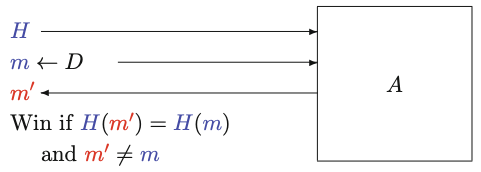
\includegraphics[width=0.35\textwidth]{img/2ndpreimage.png}
    \caption{Security game for second preimage resistance}
\end{figure}

This security game can be won by the adversary, because the domain of the message space (arbitrary length) is huge compared to the domain of the output. The output is fixed size, let's say 128. Then the domain is ``only'' $2^128$. There will be a number of collisions. 

\subsubsection{Collision Resistance}
Assume now that the domain is much larger than the co-domain. Given $H$, it should be infeasible to compute $m$ and $m'$ such that $H(m) = H(m')$.

\begin{defn}
    A hash function $H$ is \textbf{collision resistant} if it is computationally infeasible to find $m$ and $m'$ such that $H(m) = H(m')$.
    Given an output of $t$ bits, it should take $O(2^{t/2})$ time to find a collision.
\end{defn}

\begin{figure}[h!]
    \centering
    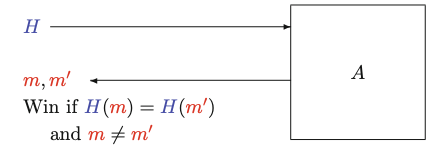
\includegraphics[width=0.35\textwidth]{img/col_resistance.png}
    \caption{Security game for collision resistance of a function}
\end{figure}

This security game can also be won by the adversary! There are several collusions: pigeonhole principle. We solved the same problem in PRFs by using a keyed version of the functions. However, we need unkeyed hash functions! This is because we need to be able to verify the integrity of the data without having the key (public use, no secret). Keyed hash functions are for security and authentication.

\begin{defn}
A function H is said to be collision resistant (by human
ignorance) or HI-CR secure if it is believed to be infeasible to write
down a collision for the function, i.e. two elements in the domain
mapping to the same element in the codomain.
\end{defn}

The probability to have a collision is $\sqrt{2^{t+1}}$ (Birthday paradox). \\

In summary, a cryptographic hash function:
\begin{enumerate}
    \item Preimage Resistant: It should be hard to find a message with
    a given hash value
    \item Second Preimage Resistant: Given one message it should be
    hard to find another message with the same hash value
    \item Collision Resistant: It should be hard to find two messages
    with the same hash value
\end{enumerate}

(1) is weaker than (2) and (3), (2) is weaker than (3). Some more terminology:

\begin{itemize}
    \item one-way = preimage + second preimage resistant
    \item weak collision resistant = second preimage resistant
    \item strong collision resistant = collision resistant
    \item OWHF = one-way hash function = preimage and second preimage resistant
    \item CRHF = collision resistant hash function = collision resistant and second preimage resistant
\end{itemize}

\subsection{Padding}
Even though the input size can be arbitrary, many hash algorithms process data in fixed-size blocks (e.g., 512-bit blocks for SHA-256). If the input data is not a multiple of the block size, padding is added to make the data fit perfectly into blocks.
Padding also helps to include the original message length in the hash calculation, which is crucial for preventing certain types of attacks (like length-extension attacks). \\

When you divide a message into smaller blocks, how can you pad it? Given an $l$ bit message $m$, and block size $b$, we want to have $m$ of length $kb$:
\[ m || \text{pad}_i(|m|, b) \]

In theory, padding can be applied at the beginning or the end. In practice, all algorithms pat at the end. \\

\subsubsection{Padding Methods}
We define 5 of them:

\begin{itemize}
    \item \textbf{Method 0:} $v = b - |m| \mod b$ and padding is $v$ zeros: $m||0^*$. In other words, the message is padded with zeros until it is a multiple of the block size
    \item \textbf{Method 1:} $v = b - (|m|+1) \mod b$ and padding is: $m||10^*$.
    \item \textbf{Method 2:} $v = b - (|m|+65) \mod b$ and padding is: $m||10^*||L$, where $L$ is a 64-bit integer encoding of $|m|$
    \item \textbf{Method 3:} $v = b - (|m|+64) \mod b$ and padding is: $m||0^*||L$
    \item \textbf{Method 4:} $v = b - (|m|+2) \mod b$ and padding is: $m||10^*1$
\end{itemize}

Any can be used, apart from method 0, but will effect security. Method 1 is also not good. \\

For SHA-256: The input message is padded by appending a 1 bit, followed by enough 0 bits, so that the total length is 64 bits short of a multiple of 512. Then, the original message length (in bits) is added as a 64-bit value at the end of the padded message.

\subsection{Merkle-Damg\aa rd Construction}
\begin{defn}
    A \textbf{compression function} is a hash function that takes an input and produces a fixed-size output. It is applied iteratively to compress larger inputs into a smaller output. After all blocks are processed, the final state becomes the output of the hash function.
\end{defn}

The MD construction is a method for building cryptographic hash functions. The construction breaks down the process of hashing into a series of steps where the input data is processed in fixed-size blocks. The key idea is to iteratively compress these blocks using a compression function.

\begin{figure}[h!]
    \centering
    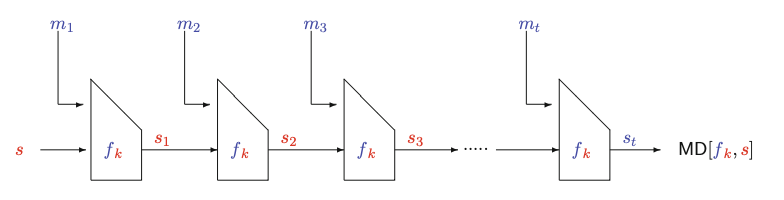
\includegraphics[width=0.5\textwidth]{img/MDconstruction.png}
    \caption{The Merkle-Damg\aa rd Construction MD$[f_k, s]$, where $s$ is the internal state}
\end{figure}

If the compression function is secure, then the hash function is secure too. 

\subsubsection{MD Algorithm}
\begin{itemize}
    \item Divide the innput message into fixed-size blocks. Apply padding if the message length is not a multiple of the block size.
    \item The process begins with an initial value (IV), a predefined set of constants.
    \item Iteratively apply the compression function $f_k$ to each block, taking the current state and block of data as input. The output of the compression function becomes the new state passed to the next iteration.
    \item After all blocks are processed, the final state becomes the final hash output.
\end{itemize}

\begin{figure}[h!]
    \centering
    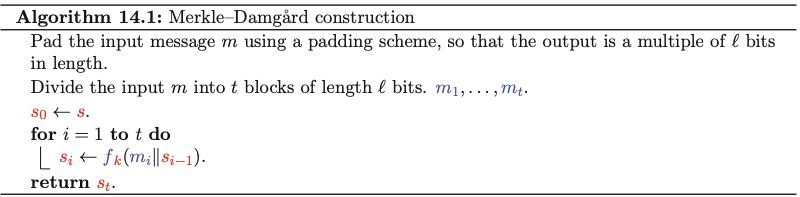
\includegraphics[width=0.6\textwidth]{img/MDalgorithm.png}
\end{figure}

\subsubsection{Benefits of MD Construction}
\begin{itemize}
\item Design makes streaming possible
\item Hash function analysis becomes compression function analysis
\item Analysis is easier because the domain of CF is finite
\end{itemize}

\subsubsection{Properties of MD Construction}
Collision resistance of the hash function depends on the padding method. Imagine there are two messages $m=0b0$ and $m'=0b00$. 
Using method 0, both of them will be mapped to $0b0000 \rightarrow$ collision.
This means that the original message can be $0b0, 0b00, 0b000, 0b0000$. All of them will be mapped to the same value.
Thus, MD-based hash function should \emph{not} use padding method 0. Use method 2 instead.

\subsubsection{Security properties under different scenarios}
\begin{enumerate}
    \item \textbf{\( s \) is fixed to an IV, \( f_k \) is also fixed:}
    \begin{itemize}
        \item \( s \) is initialized to a fixed Initial Value (IV), and \( f_k \), the compression function, is also fixed.
        \item If \( f \) is \textbf{HI-CR secure} (Highly Iterated Collision-Resistant), then the hash function \( H(m) \), constructed using the MD construction, is also collision-resistant.
        \item \textbf{Practical Use:} This describes the standard cryptographic hash functions where the IV and compression function are predefined.
    \end{itemize}
    
    \item \textbf{\( s_0 \) is a key, \( f_k \) is a fixed function:}
    \begin{itemize}
        \item Here, \( s_0 \) is treated as a \textbf{key} (instead of a fixed IV), while \( f_k \), the compression function, remains fixed.
        \item If \( f \) is \textbf{HI-CR secure}, the keyed hash function \( H_s(m) \) (where \( s_0 \) is the key) is also collision-resistant.
        \item \textbf{Practical Use:} This construction aligns with setups like HMAC, where a secret key is combined with the message for added security.
    \end{itemize}
    
    \item \textbf{\( f_k \) is from a PRF family, \( s \) is fixed:}
    \begin{itemize}
        \item In this case, \( f_k \) comes from a \textbf{Pseudorandom Function (PRF) family}, and \( s \) (the initial value) is fixed.
        \item If \( f \) is \textbf{CR secure} (Collision-Resistant), then \( H_k(m) \), constructed using the MD process, is also collision-resistant. However, this setup has limited practical implications.
        \item \textbf{Practical Use:} This is more of a theoretical observation, as using a PRF family for \( f_k \) doesn’t add significant value for hashing in practice.
    \end{itemize}
\end{enumerate}

\subsection{MD-4}
MD-family is a series of hash functions: MD construction with a (fixed) \emph{unkeyed} compression function $f$.


MD-4 (128-bit output) function f has 3 rounds of 16 steps each.

\begin{figure}[h!]
    \centering
    \begin{subfigure}{0.45\textwidth}
        \centering
        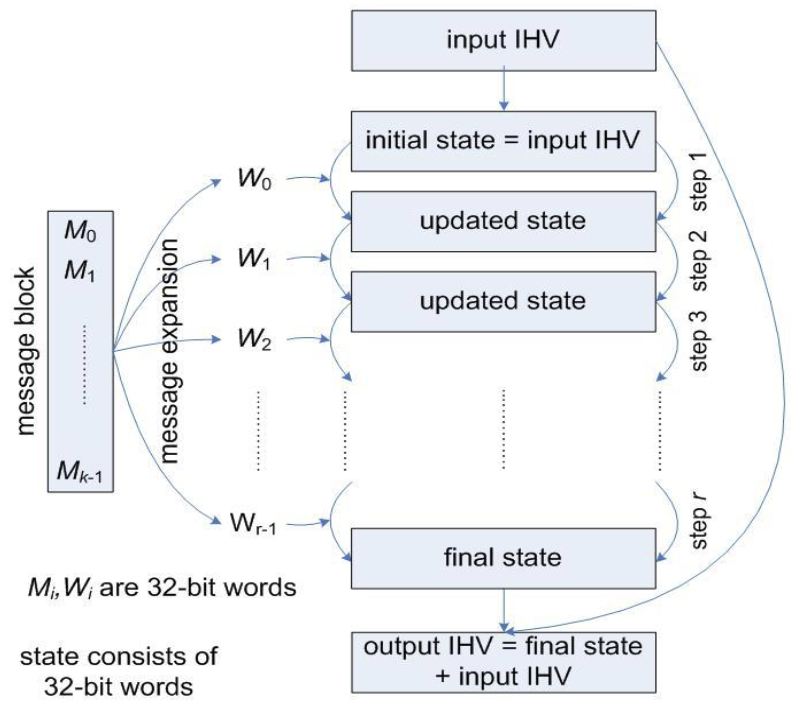
\includegraphics[width=0.9\textwidth]{img/md4.png}
        \caption{MD-4 compression function}
    \end{subfigure}
    \hfill
    \begin{subfigure}{0.45\textwidth}
        \centering
        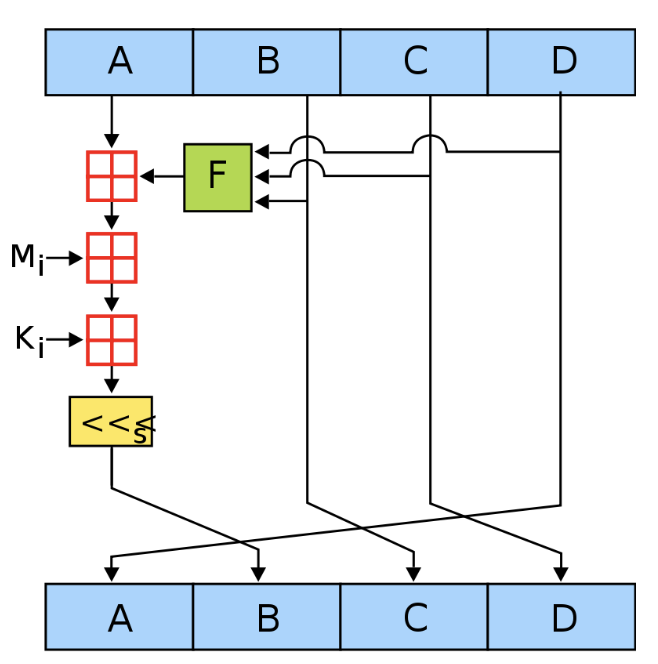
\includegraphics[width=0.9\textwidth]{img/md4steps.png}
        \caption{Steps in MD-4}
    \end{subfigure}
    \caption{MD-4 Compression Function and Steps}
\end{figure}




\subsection{Birthday Paradox}


\subsection{MAC}

\subsection{Sponge Functions}